\documentclass[10pt,a4paper]{article}

\usepackage[margin=1.9cm]{geometry}
\usepackage[T1]{fontenc}
\usepackage[utf8]{inputenc}
\usepackage{lmodern}
\usepackage{booktabs}
\usepackage{tabularx}
\usepackage{array}
\usepackage{enumitem}
\usepackage{graphicx}
\usepackage[hidelinks]{hyperref}
\usepackage[font=small,skip=4pt]{caption}
\usepackage{titlesec}
\titlespacing*{\section}{0pt}{8pt}{4pt}
\titlespacing*{\subsection}{0pt}{6pt}{3pt}
\setlength{\textfloatsep}{8pt}
\setlength{\intextsep}{6pt}

\newcolumntype{L}{>{\raggedright\arraybackslash}X}
\newcommand{\code}[1]{\texttt{#1}}
\newcommand{\ra}{$\rightarrow$}
\setlist{itemsep=2pt, topsep=4pt}

\title{RAG Assignment: Baseline Retrieval vs.\ Cross-Encoder Re-Ranking}
\author{Hritik Ranjan \quad (Roll No.\ 2025202031)}

\begin{document}
\vspace*{-1.2cm}
{\let\newpage\relax\maketitle}
\vspace{-0.6cm}

\noindent code: \href{https://github.com/HRITIK-RANJAN/RAG-BASELINE-VS-RERANKING}{https://github.com/HRITIK-RANJAN/RAG-BASELINE-VS-RERANKING}

\section*{Setup \& Environment}
\begin{itemize}
  \item \textbf{Dataset:} \emph{Netrunner Comprehensive Rules v26.03}, a 99-page rulebook with many restrictions and exceptions.
  \item \textbf{Models:} \code{all-MiniLM-L6-v2} embeddings, FAISS cosine search, \code{ms-marco-MiniLM-L-6-v2} re-ranking, and Gemini Flash Lite for answers (temperature 0).
  \item \textbf{Corpus and machine:} 602 structure-aware chunks were used. Both pipelines use the same frozen corpus.
\end{itemize}

\section{Two-Stage Retrieval}

\subsection{Pipeline 1: baseline retrieval}
The bi-encoder embeds the query and all chunks independently. FAISS returns the top 10 by cosine similarity, and the top 3 are sent to the LLM.

\subsection{Pipeline 2: advanced re-ranking}
The second pipeline re-scores those same 10 candidates with the Cross-Encoder, then sends its top 3 to the identical LLM prompt.

\section{Architecture comparison}

A \textbf{Bi-Encoder} creates independent embeddings for the query and each chunk, then compares them with cosine similarity. Chunk vectors can be computed offline, making it fast, but word relationships such as ``cannot'' or ``only if'' may be blurred.

A \textbf{Cross-Encoder} reads the query and chunk together with joint self-attention across their tokens and gives one pairwise score. This captures conditions and wording better, but requires a separate model pass for every candidate at query time.

\section{Failure Mode Analysis (Stress Testing)}

\textbf{Query set.} The final set contains 23 stress-test queries covering controls, keyword traps, exceptions, negation and buried answers. It is not a random sample.

\begin{table}[h]
\centering
\begin{tabular}{lcccc}
\toprule
 & Hit@3 & Recall@3 & MRR@10 & Mean gold rank (in top 10) \\
\midrule
Pipeline 1 (baseline)  & 0.652 & 0.514 & 0.637 & 2.29 \\
Pipeline 2 (re-ranked) & \textbf{0.696} & \textbf{0.638} & \textbf{0.687} & \textbf{2.24} \\
\bottomrule
\end{tabular}
\caption{Retrieval metrics on the 23 final queries (essential gold chunks only).}
\end{table}

By category (Hit@3 baseline \ra{} re-ranked): buried 0.40 \ra{} 0.60, control 0.83 \ra{} 1.00, exception 0.67 \ra{} 0.67, keyword trap 0.60 \ra{} 0.60, negation 0.75 \ra{} 0.50. Re-ranking moved the best gold chunk up in 5 queries, down in 6 and left it in place in 12. The two models agree only moderately on the order of the same 10 chunks (median Spearman 0.38, range $-0.20$ to 0.94).

\begin{table}[h]
\centering
\small
\begin{tabularx}{\textwidth}{lllL}
\toprule
ID & Category & Gold chunk: bi \ra{} CE rank & Query \\
\midrule
\multicolumn{4}{l}{\emph{Fixed by re-ranking}} \\
Q02 & control      & 5.2.6: \#7 \ra{} \#1 & What basic actions can the Corp always take during their turn? \\
Q29 & keyword trap & 8.1.2e: \#4 \ra{} \#1 & How does the Corp flip an installed card face up so that it starts working? \\
Q35 & buried       & 7.4.7: \#4 \ra{} \#1 & In what order are cards from the Corp's deck offered to the Runner when R\&D is breached? \\
Q41 & buried       & 7.3.8: \#4 \ra{} \#1 & If stealing an agenda would cause a breach of the same server during an ongoing breach, when does the second breach happen? \\
\multicolumn{4}{l}{\emph{Hurt by re-ranking}} \\
Q23 & negation     & 3.8.5: \#1 \ra{} \#7; 10.3.1d: \#8 \ra{} \#4 & Can the Runner have two consoles installed at the same time? \\
Q32 & keyword trap & 4.2.7: \#3 \ra{} \#4 & What happens when the Corp runs out of cards in their deck and has to draw? \\
Q36 & buried       & 7.5: \#1 \ra{} \#9 & What does the Runner do in a breach when there are no more cards left to choose from? \\
\multicolumn{4}{l}{\emph{Failing in both / not in the top 10}} \\
Q18 & negation     & 1.2.2: \#6 \ra{} \#6 & If one effect says a player must do something and another says they cannot, which applies? \\
Q34 & buried       & 7.4.6: \#4 \ra{} \#5 & While the Runner is breaching HQ, a new card enters the Corp's hand. Can the Runner access it? \\
Q12 & exception    & 1.13.13: not in top 10 & What happens to cards hosted on a card that moves from the Corp's to the Runner's score area? \\
Q42 & keyword trap & 10.1.1: not in top 10 & What happens if I have two copies of a card with the diamond symbol in play? \\
\bottomrule
\end{tabularx}
\caption{Rank shifts of the gold chunk for every final query whose outcome is not ``both ok''.}
\end{table}

\paragraph{Examples.} Q29 is a keyword trap: ``flip face up'' refers to the rule term ``rez''. Its relevant chunk moved from rank 4 to rank 1. Q02 and two buried-answer queries also moved into the top 3.

\paragraph{Exceptions and negation.} Q18's ``cannot'' rule (1.2.2) stays at rank 6 under both two-stage models; when the cross-encoder scores all 602 chunks, it ranks only 20th. For Q12, the gold chunk starts at bi-encoder rank 20, outside the top 10 candidates, so the two-stage re-ranker cannot see it.

\paragraph{Limitations.} Re-ranking also hurt: Q36 moved from rank 1 to rank 9. Q23 has two essential passages: 3.8.5 fell from rank 1 to rank 7, while 10.3.1d rose from rank 8 to rank 4---still outside the top 3. This illustrates that the best-gold metric alone can hide a harmful move of another required passage.

\begin{figure}[!htbp]
\centering
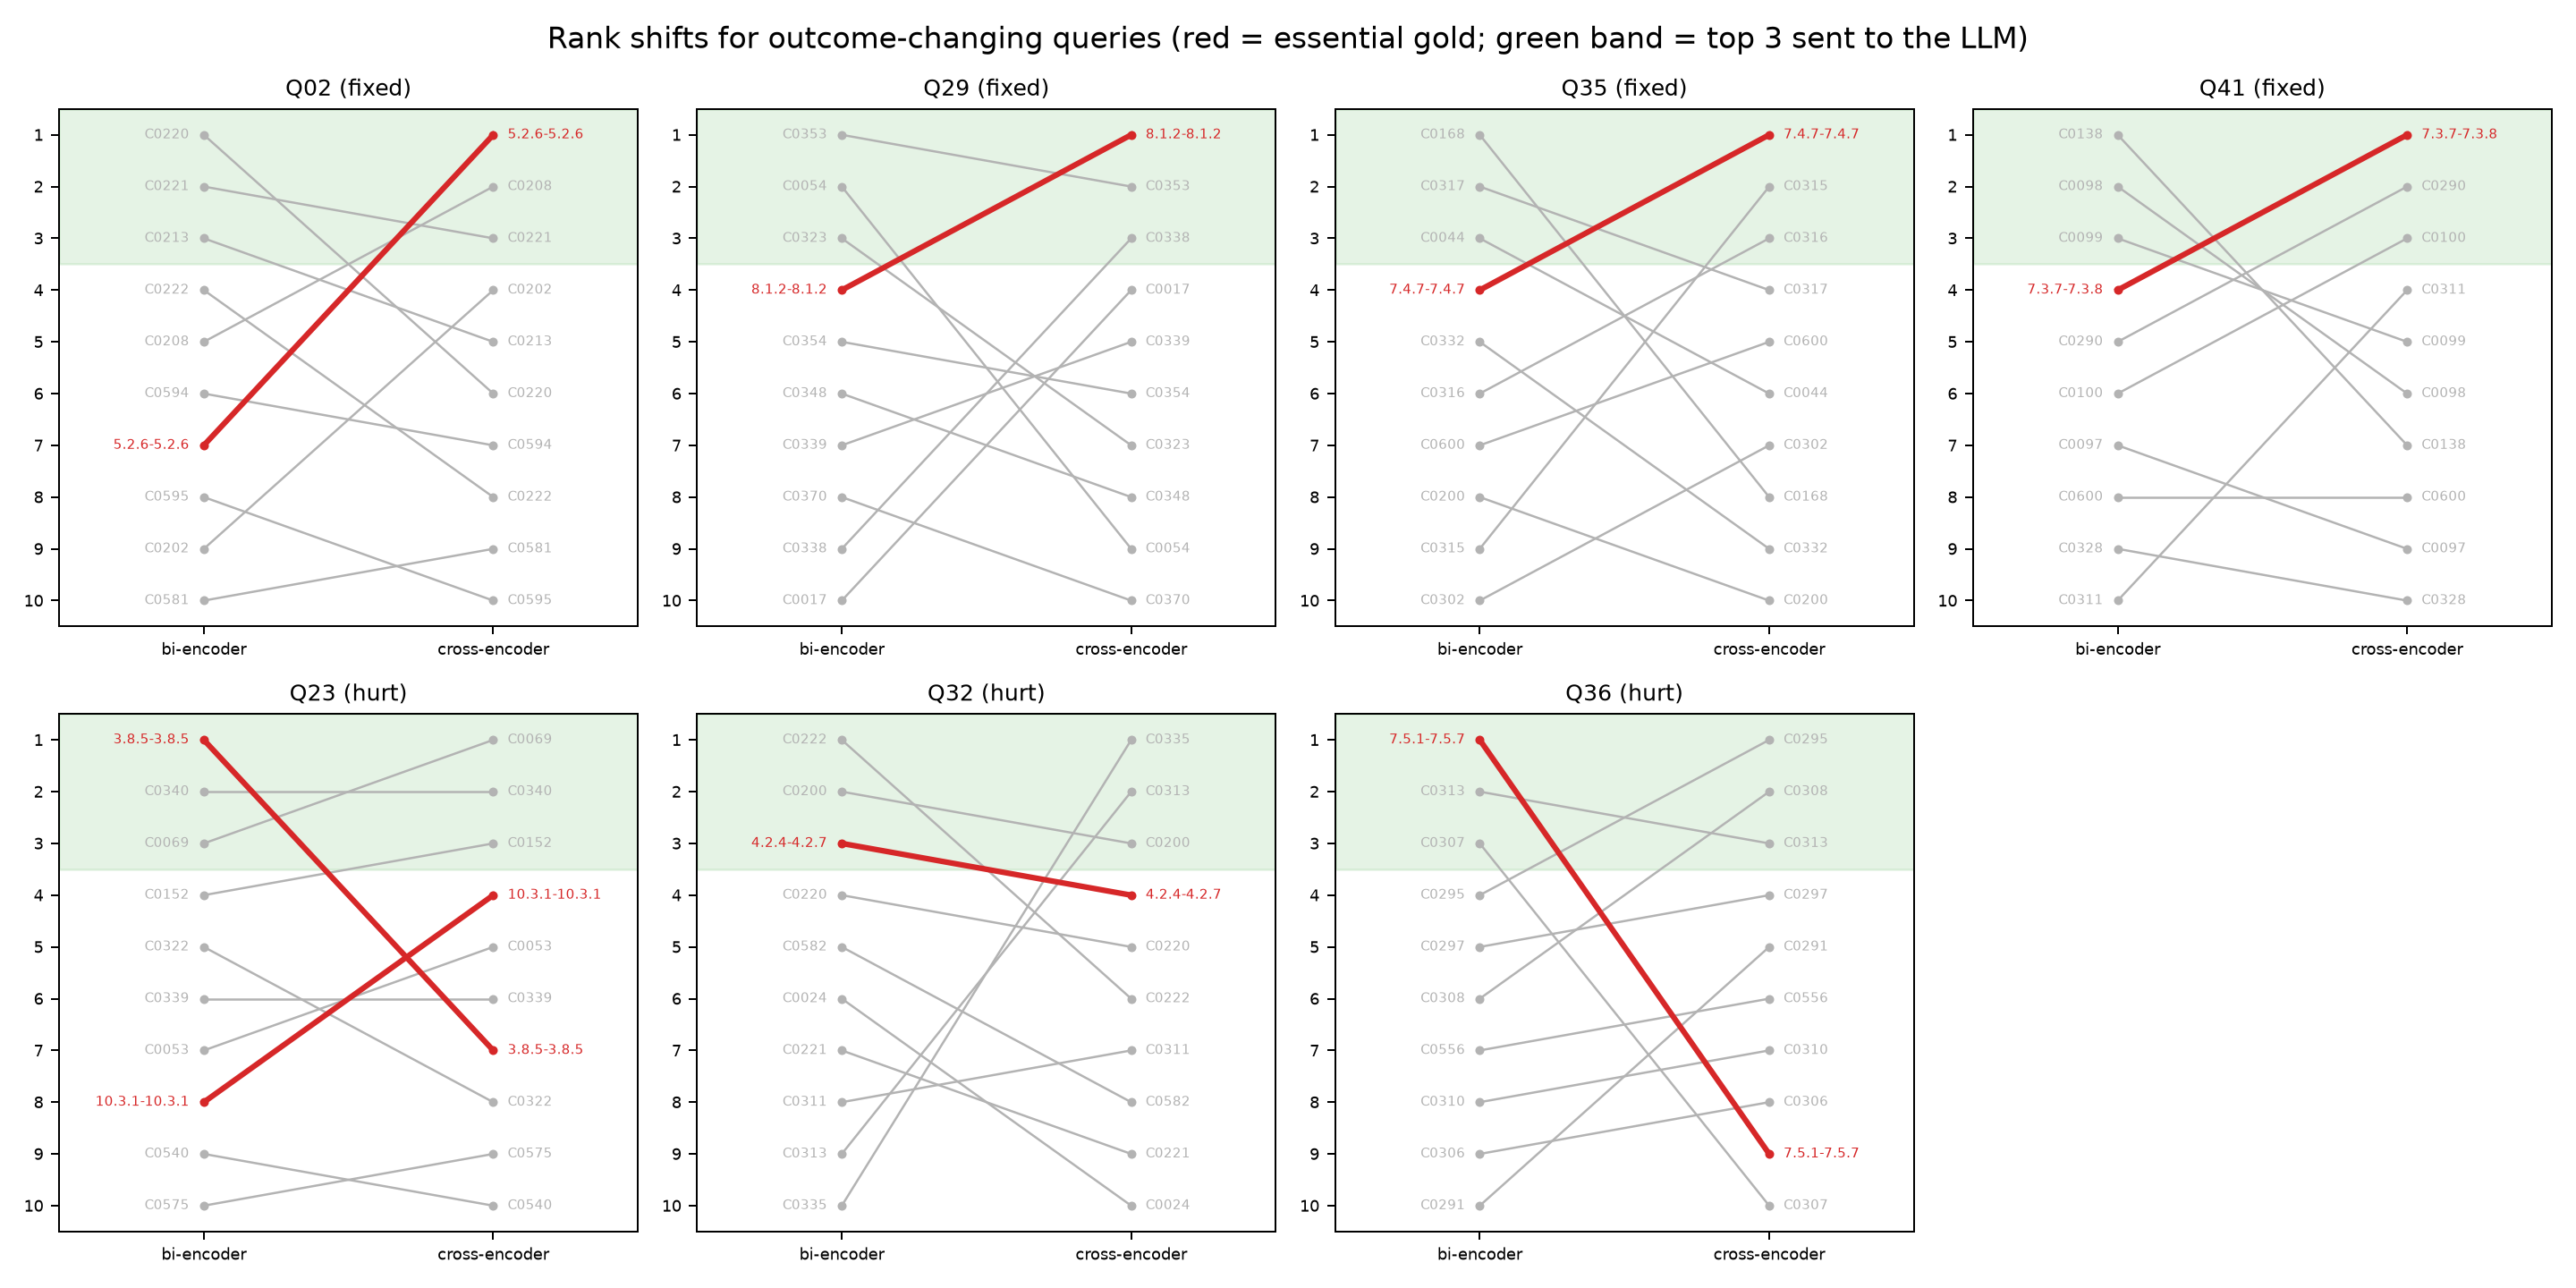
\includegraphics[width=\textwidth]{../artifacts/figures/bump_charts.png}
\caption{Rank shifts for the four fixed and three hurt queries. Red = essential gold chunk; green band = top 3 sent to the LLM.}
\end{figure}

\subsection{Answer 1 vs.\ Answer 2}

Answer~1 had 15 correct answers, 7 refusals and 1 hallucination. Answer~2 had 16 correct answers, 6 refusals and 1 hallucination. Four baseline refusals became correct after the relevant chunk entered the top 3; three correct baseline answers became refusals when re-ranking moved that chunk out. There were no `omits clause' or `misstates' cases: the refusal instruction turned missing evidence into refusals. Q34 is the only hallucination: its expected conclusion is indeed ``yes'', but both answers are labelled hallucinated because none of their supplied passages supports that claim---rule 7.4.6 was rank 4 for Pipeline 1 and rank 5 for Pipeline 2. A concrete improvement is Q29: Answer~1 refused, whereas Answer~2 used the retrieved rule to explain rezzing correctly.

\section{Latency}

Timings exclude model loading. Retrieval stages use 20 repeats over the 23 queries; the LLM uses one real call per query and pipeline, timed separately because API latency is variable.

\begin{table}[h]
\centering
\small
\begin{tabular}{lrrrrrr}
\toprule
 & \multicolumn{3}{c}{Pipeline 1 (ms)} & \multicolumn{3}{c}{Pipeline 2 (ms)} \\
\cmidrule(lr){2-4}\cmidrule(lr){5-7}
Stage & median & mean & p95 & median & mean & p95 \\
\midrule
Query encoding (bi-encoder) & 4.12 & 4.23 & 4.72 & 4.12 & 4.23 & 4.72 \\
FAISS search, top 10        & 0.02 & 0.02 & 0.03 & 0.02 & 0.02 & 0.03 \\
Cross-encoder, 10 pairs     & -- & -- & -- & 35.04 & 34.64 & 36.14 \\
\textbf{Retrieval subtotal} & \textbf{4.15} & 4.25 & 4.75 & \textbf{39.22} & 38.89 & 40.61 \\
LLM generation (Gemini)     & 1322.5 & 5036.4 & 7439.2 & 1764.6 & 5418.8 & 14826.3 \\
End-to-end                  & 1326.6 & 5040.6 & 7443.3 & 1802.3 & 5457.6 & 14865.3 \\
\bottomrule
\end{tabular}
\caption{Latency per query (Apple M4, MPS).}
\end{table}

Re-ranking itself adds about 35\,ms per query. The LLM median difference (1.32\,s for Pipeline~1 versus 1.76\,s for Pipeline~2) is API noise, not a re-ranking cost: the prompts were sent independently at different times. The means near 5\,s are driven by one 61.5\,s Pipeline~1 call (Q31) and one 31.4\,s Pipeline~2 call (Q28). Thus the 1.3\,s versus 1.8\,s end-to-end medians should not be read as the price of re-ranking; the measured local cost is 35\,ms.

\section{Why not cross-encode the whole corpus?}

The Cross-Encoder cannot precompute a score because it needs the query and chunk together. Its cost therefore grows linearly with the number of chunks: about \textbf{2.74\,ms per pair}. The Bi-Encoder first narrows the collection cheaply, leaving only 10 pairs for accurate re-ranking.

\begin{table}[h]
\centering
\begin{tabular}{rrr}
\toprule
Chunks $N$ & Cross-Encoder on all $N$ & Two-stage (encode + exact search + CE on 10) \\
\midrule
602        & 1.66\,s             & 0.04\,s \\
100,000    & 274\,s (4.6 min)    & 0.04\,s \\
1,000,000  & 2,736\,s (46 min)   & 0.07\,s \\
10,000,000 & 27,364\,s (7.6\,h)  & 0.37\,s \\
\bottomrule
\end{tabular}
\caption{Time per query (above 200k chunks: linear extrapolation; approximate indexes would make the two-stage column grow even more slowly).}
\end{table}

For this corpus, re-ranking all 602 chunks takes about 1.66\,s (the measured median), compared with about 0.04\,s for two-stage retrieval. This also measures the recall ceiling: full-corpus cross-encoding puts Q12 at rank 1 and raises Hit@3 to 0.739, versus 0.696 for the two-stage pipeline. At 1 million chunks, the same approach would take roughly 46 minutes per query. The quality gain comes at about 1.62\,s extra per query on this corpus.

\section*{Limitations}
The query set was selected for stress testing, and timings are from one machine. LLM latency is noisy; scaling figures beyond the measured corpus are extrapolations.

\end{document}
